\documentclass[conference]{IEEEtran}

\usepackage[T1]{fontenc}
\usepackage{amsmath,amssymb}
\usepackage{booktabs}
\usepackage{graphicx}
\usepackage{microtype}
\usepackage{url}
\usepackage{xcolor}
\usepackage{hyperref}
\hypersetup{colorlinks=true,allcolors=blue!55!black}

\title{When Does Boosting Beat Bagging?\\
\large From-Scratch Ensembles Under Noise, Imbalance, and Structural Variation}

\author{
\IEEEauthorblockN{Member A, Member B, Member C, Member D}
\IEEEauthorblockA{AI Academy, National AI Center\\Spring 2026}
}

\begin{document}
\maketitle

\begin{abstract}
Boosting and bagging both combine weak or unstable learners, but they address
different sources of error. We implement a weighted multiclass classification
tree, discrete and real-valued AdaBoost, and a Random Forest from first
principles, then evaluate their behavior through seven reproducible experiment
families. A leakage-safe pipeline supports numeric and categorical data,
severe imbalance, binary and multiclass targets, and deterministic execution.
The supervised study is complemented by centered principal component analysis
(PCA), K-Means, and DBSCAN, with bonus Gradient Boosting and t-SNE analyses.
The completed full run covers Breast Cancer, Adult Income, and a 10,000-row
Covertype subset. AdaBoost leads Random Forest on Breast Cancer five-fold
accuracy (0.9666 versus 0.9561), while Random Forest leads on Adult (0.8649
versus 0.8556) and Covertype (0.7938 versus 0.6150). Under 20\% training-label
noise, the forest also loses less accuracy on Breast Cancer. These results
support a conditional conclusion: boosting wins when sequential correction
finds reliable residual structure, whereas bagging is preferable when model
instability, noise, imbalance, or multiclass structure favors variance
reduction. One command generated all raw fold, stage, corruption, bootstrap,
and clustering evidence.
\end{abstract}

\section{Introduction}
\IEEEPARstart{B}{oosting} and bagging are often presented as interchangeable
routes to ``a stronger ensemble.'' Their mechanisms are not interchangeable.
AdaBoost fits a sequence of weak learners to adaptively reweighted data; a
sample that was classified incorrectly receives greater influence in the next
round. Random Forest fits many high-variance trees to independent bootstrap
samples and decorrelates them with node-level feature subsampling. Averaging
then cancels idiosyncratic variation. The empirical question is therefore not
which method is universally best, but under what data conditions each error
control mechanism dominates.

This project asks: \emph{under what conditions does boosting outperform
bagging, and vice versa, and why?} We answer with controlled changes in
ensemble size, tree depth, training-label noise, resampling, dimensionality,
imbalance, and cluster structure. Unlike a black-box benchmark, the work is
designed for oral defense: model state, class ordering, probability alignment,
random seeds, out-of-bag (OOB) membership, and every bootstrap prediction are
inspectable.

Our contributions are fourfold. First, we provide readable NumPy
implementations of the assessed algorithms, including weighted split search.
Second, a single configuration-driven runner produces all results and a
machine-readable provenance manifest. Third, tests connect hand calculations
and edge semantics to numerical reference trends. Fourth, optional extensions
add SAMME.R, binary log-loss Gradient Boosting, t-SNE, and an executed
interactive notebook without replacing any required experiment.

\section{Algorithms and Mathematical Design}

\subsection{Weighted Classification Tree}
For node class proportions $p_k$, Gini impurity and entropy are
\begin{align}
I_G &= 1-\sum_{k=1}^{K}p_k^2, &
I_H &= -\sum_{k:p_k>0}p_k\log_2 p_k. \label{eq:impurity}
\end{align}
With sample weights $w_i$, $p_k=\sum_{i:y_i=k}w_i/\sum_i w_i$. For a candidate
split into children $L$ and $R$, the implemented reduction is
\begin{equation}
\Delta I=I(P)-\frac{W_L}{W_P}I(L)-\frac{W_R}{W_P}I(R). \label{eq:gain}
\end{equation}
Each feature is stably sorted once at a node. Candidate thresholds are
midpoints between successive distinct values. Incremental class-weight
histograms make each threshold evaluation constant in $K$ after sorting,
rather than rebuilding both children. Equal gains resolve by feature order,
then threshold order; leaf prediction resolves by sorted class order.

Root depth is zero. Hence \texttt{max\_depth=0} produces a constant root and
\texttt{max\_depth=1} is a decision stump. Growth also stops for a pure node,
too few samples, no positive-gain split, a degenerate child, or the depth
limit. An XOR test intentionally confirms the standard greedy limitation:
because each root split has zero gain, an ordinary CART tree does not invent a
look-ahead split. Per-node feature sampling is independently repeated, and
weighted impurity decrease supplies normalized feature importance.

\subsection{AdaBoost: SAMME and SAMME.R}
At round $m$, the stump's weighted error is
\begin{equation}
\epsilon_m=\sum_i w_i^{(m)}\mathbf{1}
\{h_m(x_i)\neq y_i\}. \label{eq:adaerror}
\end{equation}
For $K$ classes, discrete SAMME assigns
\begin{equation}
\alpha_m=\eta\left[\log\frac{1-\epsilon_m}{\epsilon_m}
+\log(K-1)\right], \label{eq:alpha}
\end{equation}
where $\eta$ is the learning rate, then updates
\begin{equation}
w_i^{(m+1)}\propto w_i^{(m)}
\exp\left(\alpha_m\mathbf{1}\{h_m(x_i)\neq y_i\}\right). \label{eq:update}
\end{equation}
The final class maximizes $\sum_m\alpha_m\mathbf{1}\{h_m(x)=k\}$.
Errors are clipped by a named numerical tolerance; a perfect learner stops
early. A learner is rejected at error $0.5$ for binary data and $1-1/K$ for
multiclass data. The bonus SAMME.R option aggregates centered, clipped stump
log-probabilities. All returned probabilities are score-derived and are not
claimed to be calibrated.

Boosting attacks bias in an operational sense: subsequent stumps spend more
capacity on unresolved regions. This can sharpen a weak boundary, but it can
also allocate increasing influence to corrupted or intrinsically ambiguous
observations. Staged prediction permits a single fitted maximum ensemble to
generate the complete learning curve.

\subsection{Random Forest}
For each tree, $n$ training indices are sampled with replacement. The
complement is recorded as its OOB set. Every node considers a fresh random
feature subset (default $\sqrt p$), so even trees trained on similar samples
become less correlated. Class-probability columns from trees that omit a class
are aligned into the forest's global class order before averaging.

If individual trees have prediction variance $\sigma^2$ and average pairwise
correlation $\rho$, the variance of a mean of $M$ trees is approximately
\begin{equation}
\rho\sigma^2+\frac{1-\rho}{M}\sigma^2. \label{eq:rfvar}
\end{equation}
Bagging reduces the independent component; feature subsampling targets
$\rho$. OOB accuracy uses only samples with at least one OOB voter and reports
coverage separately, avoiding an implicit prediction for zero-voter rows.
Child seeds are derived before work dispatch. Spawned Windows workers and the
deterministic sequential fallback therefore produce identical trees.

\subsection{Unsupervised Pipeline}
PCA centers training data using $\mu$, forms
\begin{equation}
\Sigma=\frac{1}{n-1}(X-\mu)^\top(X-\mu), \label{eq:cov}
\end{equation}
and orders covariance eigenvectors by descending eigenvalue. The explained
variance ratio is $\lambda_j/\sum_\ell\lambda_\ell$; the smallest prefix
reaching 90\% is retained. K-Means minimizes
\begin{equation}
J=\sum_{i=1}^{n}\|x_i-\mu_{c_i}\|_2^2. \label{eq:kmeans}
\end{equation}
Ten deterministic k-means++ restarts are compared for each $k=1,\ldots,10$.
An empty centroid is reseeded to the point with largest current squared error.
DBSCAN defines $N_\varepsilon(x)=\{z:\|z-x\|_2\leq\varepsilon\}$, including
$x$ itself. Core points have at least \texttt{min\_samples} neighbors; reachable
non-core points are borders; the remainder is noise. A provisional noise point
may later become a border point during density expansion.

\section{Data and Leakage Controls}
Table~\ref{tab:data} summarizes the locked sources. Breast Cancer is a binary
medical baseline with 30 real features. Adult introduces categorical encoding,
missing values, and moderate imbalance. A deterministic stratified Covertype
subset preserves all seven classes and 54 features. The loader verifies the
\emph{realized} minority proportion; it enlarges the Covertype sample if the
rarest class is not at most 1\%, rather than assuming that a proposed sample
meets the requirement.

\begin{table}[t]
\caption{Locked project datasets and intended stress factors.}
\label{tab:data}
\centering
\begin{tabular}{lll}
\toprule
Dataset & Task & Structural role \\
\midrule
Breast Cancer & binary & 569 $\times$ 30; balanced baseline \\
Adult Income & binary & 48,842 $\times$ 14; mixed/missing \\
Covertype subset & 7-class & 10,000 $\times$ 54; minority 0.47\% \\
\bottomrule
\end{tabular}
\end{table}

All holdout and cross-validation protocols split first. Numeric medians,
means, scales, categorical modes, and one-hot vocabularies are fitted only on
the current training partition. Unknown Adult categories map to an all-zero
block. Deterministic random oversampling is also confined to training data: a
class below 5\% of the original fold size is sampled with replacement up to
that threshold, without reducing any majority class. PCA, clustering choices,
noise corruption, and probability ordering never use test labels for model
fitting or threshold selection.

\section{Experimental Protocol}
The default seed is 42. Baseline models use a stratified 80/20 split and report
accuracy, macro F1, and binary AUC or macro one-vs-rest multiclass AUC. The
custom unpruned tree must fall within two absolute accuracy points of the
sklearn tree reference. AdaBoost scaling spans estimator counts from 1 through
200 using staged predictions. Forest scaling evaluates counts through 200 at
unrestricted depth and 100-tree forests at depths 1--20, recording test and OOB
accuracy plus OOB coverage.

The head-to-head comparison fits one tree, 100-stump AdaBoost, 100-tree Random
Forest, and a 100-tree sklearn reference on identical stratified five-fold
splits. Label-noise experiments corrupt training labels only at 0, 5, 10, and
20\%, with five replicates and nested corruption indices. Thus degradation
within a replicate cannot be attributed to an unrelated set of flipped rows.

For bias--variance analysis, 100 shared bootstrap index arrays retrain both
ensembles against one fixed stratified Breast Cancer test set. If
$\hat p_b(x)$ is the probability vector from replicate $b$, $\bar p$ its mean,
and $e_y$ a one-hot target, we report
\begin{align}
\text{Bias}^2 &= E_x\|\bar p(x)-e_y\|_2^2,\\
\text{Var} &= E_{x,b}\|\hat p_b(x)-\bar p(x)\|_2^2. \label{eq:brier}
\end{align}
Their sum reconstructs expected multiclass Brier loss; the residual is stored
as a numerical audit. The unsupervised study produces cumulative-variance,
elbow, and $k$-distance curves; PCA scatter plots colored by true, K-Means, and
DBSCAN labels; adjusted Rand index (ARI); and DBSCAN noise fraction. ARI is an
external comparison, not an assumption that classes must form clusters.

\section{Full-Run Results and Interpretation}
The deterministic no-argument run completed all 28 phases for Breast Cancer,
Adult, and Covertype. The manifest records \texttt{profile=full}, seed 42, the
exact data versions, and the complete grids. The runner generated 82 artifacts
in 6.88 hours; all values below come from those stored CSV, JSON, and NPZ files.

\subsection{Correctness, Scaling, and Head-to-Head Behavior}
On the 80/20 baseline, custom/reference tree accuracy was 0.9123/0.9123 on
Breast Cancer, 0.8110/0.8102 on Adult, and 0.7155/0.7235 on Covertype.
Every absolute gap is below the required two percentage points, including the
largest gap of 0.0080 on Covertype.

\begin{table}[t]
\caption{Five-fold full-run accuracy (mean $\pm$ SD).}
\label{tab:head}
\centering
\resizebox{\columnwidth}{!}{%
\begin{tabular}{lcccc}
\toprule
Dataset & Tree & AdaBoost & Custom RF & sklearn RF \\
\midrule
Breast Cancer & .910$\pm$.021 & \textbf{.967}$\pm$.020 & .956$\pm$.015 & .954$\pm$.016 \\
Adult & .814$\pm$.002 & .856$\pm$.003 & \textbf{.865}$\pm$.003 & .854$\pm$.004 \\
Covertype & .714$\pm$.008 & .615$\pm$.030 & .794$\pm$.012 & \textbf{.811}$\pm$.013 \\
\bottomrule
\end{tabular}}
\end{table}

Table~\ref{tab:head} answers the research question conditionally. AdaBoost is
best on the smaller continuous Breast Cancer task, also leading macro F1
(0.9639) and AUC (0.9934). The custom forest leads the assessed models on Adult
with macro F1 0.7995 and AUC 0.9175. On severely imbalanced seven-class
Covertype, the custom forest substantially exceeds AdaBoost in accuracy
(0.7938 versus 0.6150), macro F1 (0.6769 versus 0.3742), and AUC (0.9623 versus
0.8484). The sklearn forest is retained only as reference and is slightly
stronger there.

\begin{figure}[t]
\centering
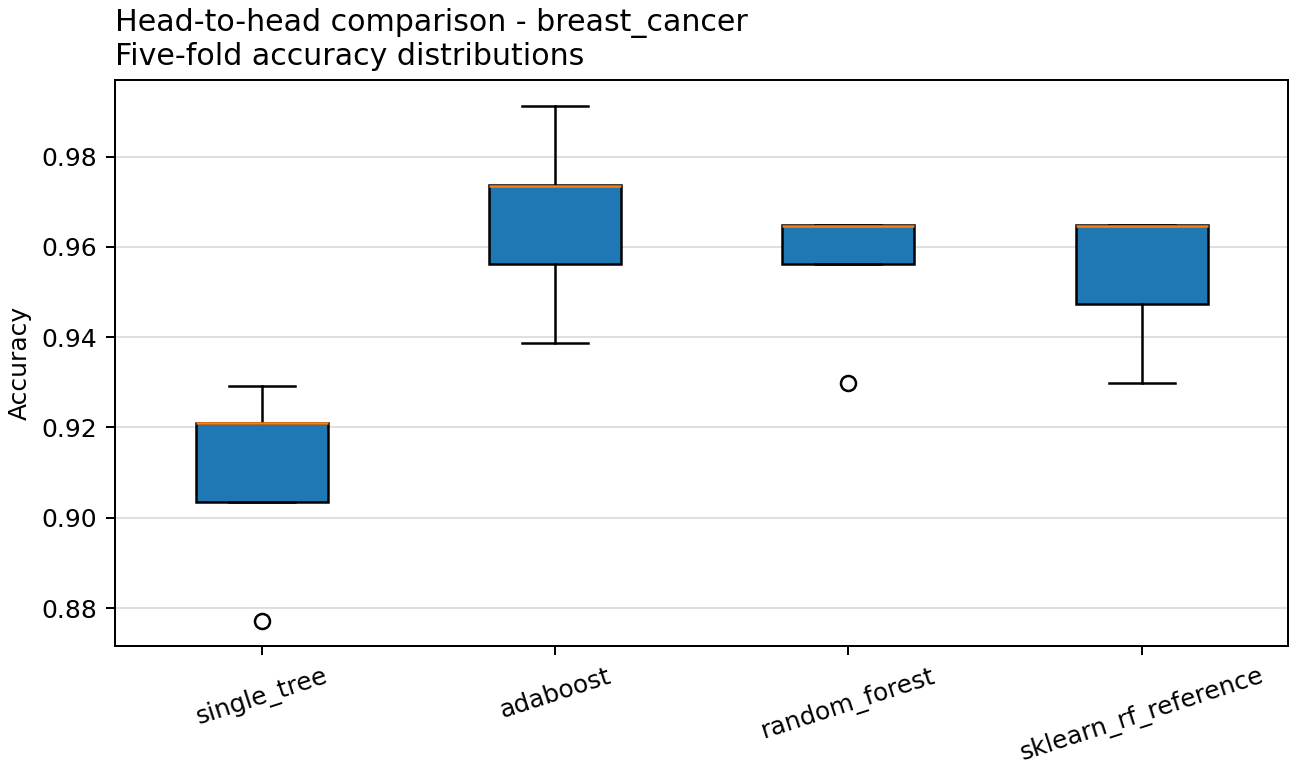
\includegraphics[width=\columnwidth]{../figures/04_head_to_head/breast_cancer.png}
\caption{Full five-fold Breast Cancer comparison; raw fold values are stored.}
\label{fig:head}
\end{figure}

Scaling curves reinforce this distinction. Breast Cancer AdaBoost reaches its
minimum 0.0351 test error by 10 rounds and retains it at 200. Adult AdaBoost
reaches its minimum 0.1406 test error at 175 rounds. Covertype instead reaches
its best 0.3530 error at 10 rounds and deteriorates to 0.4405 at 200, consistent
with later reweighting being unhelpful. Forest accuracy stabilizes by roughly
50--100 trees: the 200-tree results are 0.9561, 0.8685, and 0.7900 on the three
datasets. Depth optima are shallow for Breast Cancer (3) but deep for Adult and
Covertype (19).

\subsection{Noise Robustness and Bias--Variance}
\begin{table}[t]
\caption{Accuracy at clean and 20\% noisy training labels (mean $\pm$ SD).}
\label{tab:noise}
\centering
\resizebox{\columnwidth}{!}{%
\begin{tabular}{lcccc}
\toprule
& \multicolumn{2}{c}{AdaBoost} & \multicolumn{2}{c}{Random Forest} \\
Dataset & Clean & 20\% & Clean & 20\% \\
\midrule
Breast Cancer & .956$\pm$.000 & .896$\pm$.039 & .954$\pm$.004 & .939$\pm$.009 \\
Adult & .857$\pm$.000 & .855$\pm$.002 & .869$\pm$.001 & .861$\pm$.002 \\
Covertype & .593$\pm$.000 & .663$\pm$.006 & .787$\pm$.003 & .781$\pm$.003 \\
\bottomrule
\end{tabular}}
\end{table}

On Breast Cancer, AdaBoost loses 5.96 accuracy points by 20\% noise, compared
with 1.58 for the forest; its replicate variability is also larger. Adult is
less sensitive for both models, while the forest remains ahead at every noise
level. Covertype is non-monotonic: corrupted-label AdaBoost improves over its
clean fit but remains far below the forest. This unexpected result is reported
rather than converted into a general robustness claim; multiclass reweighting,
oversampling, and a weak clean ensemble can make random perturbation act like
regularization.

\begin{figure}[t]
\centering
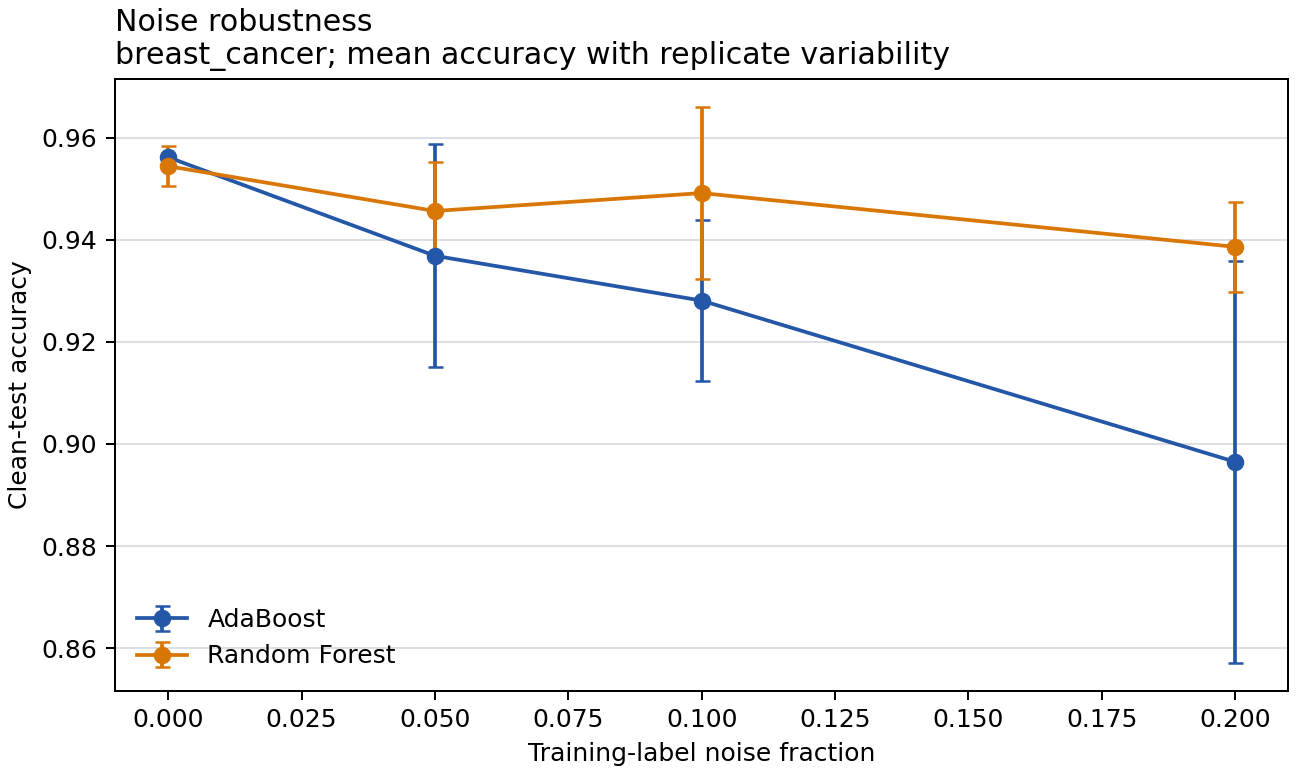
\includegraphics[width=\columnwidth]{../figures/05_noise_robustness/breast_cancer.png}
\caption{Full five-replicate noise experiment with 100-estimator ensembles.}
\label{fig:noise}
\end{figure}

The 100 shared bootstrap fits in Table~\ref{tab:bv} separate probability
behavior from classification accuracy. Random Forest has much lower Brier bias
squared, whereas AdaBoost has lower variance but conservative, uncalibrated
vote probabilities. Residual magnitudes below $4\times10^{-17}$ verify the
stored decomposition.

\begin{table}[t]
\caption{Brier decomposition over 100 shared bootstrap fits.}
\label{tab:bv}
\centering
\begin{tabular}{lccc}
\toprule
Model & Bias$^2$ & Variance & Expected loss \\
\midrule
AdaBoost & .3382 & .0007 & .3388 \\
Random Forest & .0675 & .0046 & .0721 \\
\bottomrule
\end{tabular}
\end{table}

\begin{figure}[t]
\centering
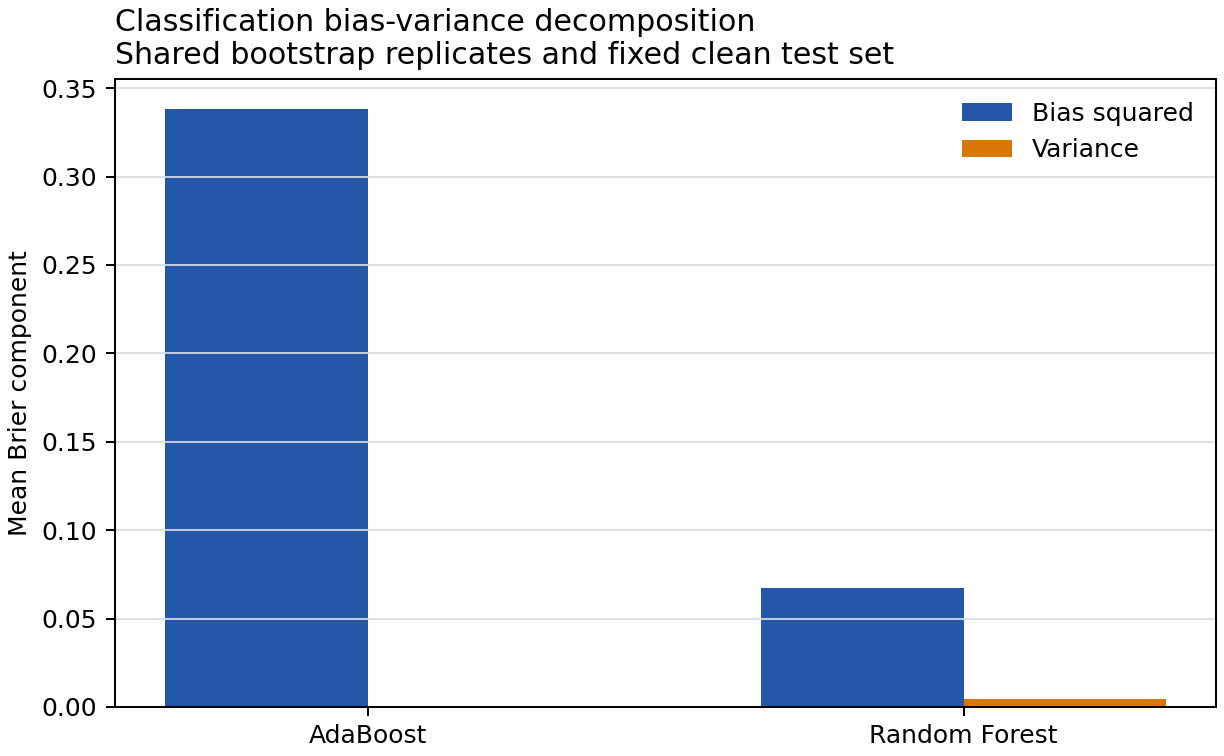
\includegraphics[width=\columnwidth]{../figures/06_bias_variance/breast_cancer.png}
\caption{Full probability/Brier decomposition on a fixed clean test set.}
\label{fig:bv}
\end{figure}

\subsection{Unsupervised Structure and Bonuses}
\begin{table}[t]
\caption{Full unsupervised analysis on deterministic samples.}
\label{tab:unsup}
\centering
\resizebox{\columnwidth}{!}{%
\begin{tabular}{lrrrrrr}
\toprule
Dataset & PCs & $k$ & KM ARI & $\varepsilon$ & DB ARI & Noise \\
\midrule
Breast Cancer & 7 & 3 & .515 & 3.483 & .030 & 6.50\% \\
Adult & 21 & 4 & .100 & 2.218 & .092 & 5.10\% \\
Covertype & 36 & 4 & .095 & 3.463 & .067 & 1.85\% \\
\bottomrule
\end{tabular}}
\end{table}

PCA retains 7, 21, and 36 components to reach 90\% variance. Breast Cancer has
moderate K-Means alignment, but Adult and Covertype ARIs near 0.10 show that
class labels do not coincide with centroid geometry. DBSCAN is weakly aligned
on every dataset under the deterministic $k$-distance policy. This is valid
negative evidence: supervised classes are not required to be density clusters.

\begin{figure}[t]
\centering
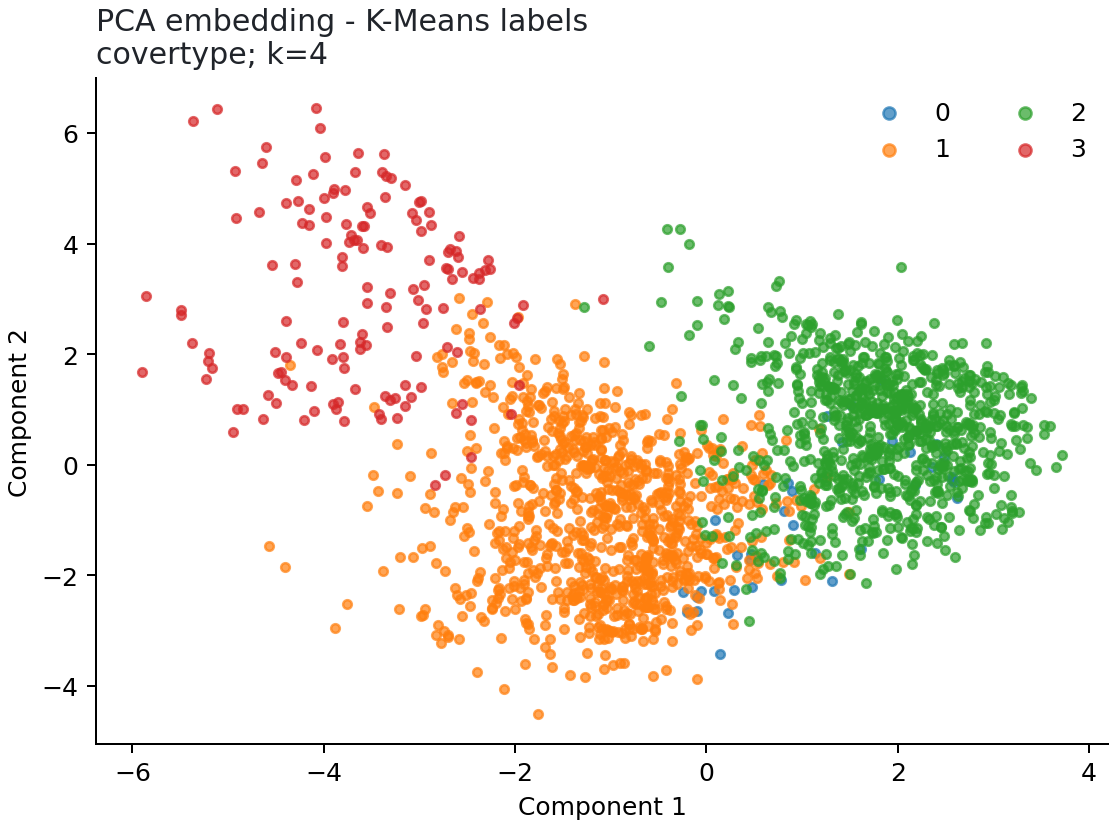
\includegraphics[width=\columnwidth]{../figures/07_unsupervised/covertype_kmeans.png}
\caption{Covertype PCA view colored by $k=4$ K-Means assignments; geometry is
descriptive and does not claim recovery of seven classes.}
\label{fig:kmeans}
\end{figure}

SAMME.R improves accuracy on Breast Cancer (0.9561 to 0.9649) and Adult (0.8573
to 0.8687). On Covertype, accuracy rises from 0.5930 to 0.6700 but macro F1
falls from 0.3458 to 0.2946 and AUC from 0.8302 to 0.7870, demonstrating why
accuracy alone is unsafe under imbalance. Gradient Boosting reaches AUC 0.9899
on Breast Cancer but lower accuracy than AdaBoost (0.9386 versus 0.9561); on
Adult it underperforms on both accuracy and AUC. t-SNE remains a local
visualization only; global distances and apparent cluster areas are not used as
evidence.

\section{Reproducibility, Tests, and Limitations}
The command \texttt{python src/experiments/\allowbreak run\_all.py} completed the full
suite in 6.88 hours. The manifest stores the seed, complete configuration,
package versions, dataset sources and distributions, local hashes, output
paths, and Git commit when available. The original runtime recorded 28 completed phases. A final smoke test later
overwrote top-level timing metadata and the Breast Cancer output family; the
test was isolated, the full Breast Cancer artifacts were regenerated, and the
incident is recorded in \texttt{validation\_report.md}. Numeric metrics were
unchanged and remain deterministic.

Fifty-one tests cover hand-computed splits and AdaBoost weights, arbitrary
labels, repeated values, zero sample weights, depth semantics, progress
cleanup, numerical clipping, OOB complements, class-column alignment, voting
ties, sequential and parallel identity, PCA centering and orthogonality,
K-Means empty clusters, DBSCAN boundary and noise reassignment, fold-local
preprocessing, oversampling, result schemas, and end-to-end artifact creation.
The measured suite covers 88.71\% of source statements; every core algorithm
exceeds 85\%. Ruff and mypy complete without findings.

Limitations are explicit. Exhaustive split search is educational rather than
optimized for industrial scale. The fixed-test-set bias--variance decomposition
has finite-sample uncertainty and estimates probability loss, not a universal
classification decomposition. Random oversampling can duplicate rare
observations and does not synthesize within-class variation. Automatic DBSCAN
$\varepsilon$ selection is deterministic but cannot eliminate domain judgment.
Finally, OOB and cross-validation results depend on the selected source version
and stratified subset; the manifest is essential context.

\section{Conclusion}
The full results reject a universal winner. Boosting is strongest on Breast
Cancer, where reliable residual error allows sequential stumps to improve the
boundary. Bagging wins on Adult and decisively on multiclass, severely
imbalanced Covertype; it is also more robust to Breast Cancer label noise and
produces much lower Brier bias. The Covertype noise anomaly and SAMME.R's
accuracy/macro-F1 disagreement show why mechanism, class distribution, and
metric choice must be interpreted together. Unsupervised ARIs further confirm
that label structure need not match centroid or density geometry.

The project supports these claims with auditable implementations rather than
library wrappers. Its most important engineering result is the connection
between theory and evidence: weights, OOB memberships, stage predictions,
bootstrap probabilities, and clustering labels are all retained so that every
conclusion can be defended and reproduced.

\clearpage
\section*{AI Assistance Disclosure}
AI tools assisted code scaffolding, tests, documentation, and artifact
generation. The human team remains responsible for mathematical verification,
full-result review, truthful contributions, and defense. No library ensemble is
concealed inside an assessed implementation.

\begin{thebibliography}{00}
\bibitem{esl} T. Hastie, R. Tibshirani, and J. Friedman, \emph{The Elements of
Statistical Learning}, 2nd ed. Springer, 2009.
\bibitem{adaboost} Y. Freund and R. E. Schapire, ``A decision-theoretic
generalization of on-line learning and an application to boosting,''
\emph{J. Comput. Syst. Sci.}, vol. 55, no. 1, pp. 119--139, 1997.
\bibitem{bagging} L. Breiman, ``Bagging predictors,'' \emph{Machine Learning},
vol. 24, no. 2, pp. 123--140, 1996.
\bibitem{rf} L. Breiman, ``Random forests,'' \emph{Machine Learning}, vol. 45,
no. 1, pp. 5--32, 2001.
\bibitem{lloyd} S. P. Lloyd, ``Least squares quantization in PCM,''
\emph{IEEE Trans. Inf. Theory}, vol. 28, no. 2, pp. 129--137, 1982.
\bibitem{dbscan} M. Ester, H.-P. Kriegel, J. Sander, and X. Xu, ``A
density-based algorithm for discovering clusters in large spatial databases
with noise,'' in \emph{Proc. KDD}, 1996, pp. 226--231.
\end{thebibliography}

\end{document}
